\documentclass[a4paper]{article}
\usepackage[utf8]{inputenc}
\usepackage[english]{babel}
%\usepackage[sc]{mathpazo}
%\linespread{1.05}         % Palatino needs more leading (space between lines)
\usepackage[T1]{fontenc}
%\usepackage[pdftex]{color,graphicx}
%\usepackage{colortbl}
%\usepackage{pdfpages}
\usepackage{fancyhdr}
%\usepackage{amsmath} % math environment
%\usepackage{listings}
\usepackage{xcolor, colortbl}
\usepackage{graphicx}
\usepackage{pdfpages}
\usepackage{setspace} % text spacing options
\usepackage{textcomp} % text symbols
\usepackage{multicol}
\usepackage{calc}
\usepackage{rotating}

%temp
\usepackage{lipsum}

\pagestyle{fancy}

%Define commands
\newcommand{\systemname}{Jenkins validated merging}
\newcommand{\groupname}{Team $\Delta$}
\newcommand{\groupmembers}{
	Andreas Frisch \{andreas.frisch@gmail.com\}, \\
	Esben Skaarup \{esben.skaarup@gmail.com\}, \\
	Alexander W. Uldall \{morpmex@gmail.com\} \\
	Ronni Elken Lindsgaard \{ronni.lindsgaard@gmail.com\}, \\
	~
}

%Define colors
\definecolor{Gray}{gray}{0.8}
\definecolor{DarkGray}{gray}{0.4}

\lhead{Project Course: Development Studio}
\chead{}
\rhead{\systemname}
\lfoot{}
\cfoot{\thepage}
\rfoot{}

%Start section numbering from 0
\setcounter{section}{-1}

\begin{document}
\begin{titlepage}
	% Title
	\begin{center}
		\vspace*{4cm}
		\rule{\linewidth}{0.5mm}\\[0.4cm]
		{\huge \bfseries \systemname}
		\rule{\linewidth}{0.5mm}
	\end{center}
	\begin{flushleft}
		{
			\Large Project Course: Development Studio \\[0.1cm]
			{\it Assignment 3 - sprint 2}
		}
	\end{flushleft}
	\vspace*{4cm}
	
	% Authors
	\begin{flushleft}
		{\Large \groupname :} \\[0.1cm]
		{\Large \groupmembers} \\[0.3cm]
		{\Large \today}
	\end{flushleft}
\end{titlepage}
\newpage
\onehalfspacing
\setcounter{tocdepth}{2}
%\tableofcontents
%newpage

\section{This hand-in}
This assignment is written as part of the course {\it Project Course: Development Studio} at DIKU.

This assignment concerns itself with our results from the second sprint.
Furthermore we will briefly discuss the lessons learned and how they affect our
upcoming sprint.

Our customer, Praqma, wants a plug-in for the continuous delivery facilitator
Jenkins, which allows Jenkins to rollback broken commits, thus maintaining an
unpolluted, pristine, company truth repository.

Our code and backlogs can be found at https://github.com/pcds2013-team-delta/pretest-commit-plugin

\section{This sprint}
This section will consist of three different yet related subjects. Firstly we
will discuss our sprint goals for this sprint -- that is the customer-related
goals and should be seen in addition to the course-related goals specified by
the assignment description. Secondly we will discuss briefly how this sprint
turned out -- what worked and what did not. Lastly we will briefly discuss what
we learned from this sprint and how we can apply that to the coming sprint.

\subsection{Sprint goals}
\label{sec:goal}
Each sprint our customer determines a simple goal which all the tasks revolve
around. Determining whether or not a given sprint was a success can be boiled
down to whether or not we achieved this goal.

For this sprint the overall goal was to enable a successful round-trip in a
sunshine scenario. In our world, a sunshine scenario is when a user submits a
commit which does not result in merge conflicts or failed builds. In such a
scenario a successful round-trip would be comprised of the following steps
\begin{enumerate}
	\item User commits changeset to remote repository.
	\item Jenkins registers this commit and starts a build.
		\begin{enumerate}
			\item Jenkins gets current base from company truth
			\item Jenkins merges current base with changeset
			\item Jenkins does what it has been set up to do\footnote{Compilation,
				Testing, Code Coverage, whatever the user has set up.}.
		\end{enumerate}
	\item Build is successful.
	\item Jenkins pushes original changeset to company truth.
\end{enumerate}

This setup requires three SCM repositories. Firstly we need a company truth
repository, second we need a repository connected to Jenkins and lastly each
client would need a private repository as is standard for distributed version
control systems. All of this requires very little setup, as all we require is
for the clients to change one of their remote directions from company truth to
Jenkins, so when they commit changes, Jenkins will now receive the changeset instead of company truth.

At the time of writing we are able to complete such a round-trip successfully.

\subsection{Sprint review}
\label{sec:review}
\begin{figure}
	\centering
	\includegraphics[width=\textwidth/2]{img/burndown.png}
	\caption{A burnup graph of our second sprint. Referring to section
	\ref{sec:review}, remember that this graph is a bit misleading as to the
	success of the sprint.}
	\label{fig:burnup}
\end{figure}

Most of our tasks for this sprint relates to the sprint goal at hand, described
in section \ref{sec:goal}. Some tasks, however, are meant as preparations for
sprints to come, most of which are considered either ``could have'' or ``should
have''. This sprint, as the last, we followed our idea of having too many story
points in the sprint backlog\footnote{Having sprints span a lot of time
introduces a lot of unpredictability, why we introduced the notion of having
some slack in both directions. Extra tasks if we got too much time and
prioritized tasks for when we have too little. This allows us to avoid adding
tasks to the sprint backlog during a sprint, which is against the sprint ideal}, and this week we needed this extra
leeway, as the sprint goal took more time to complete than we expected. 

Furthermore, for this sprint most of the tasks were hard to separate in a nice
fashion. This meant that our sprint tasks were more strongly related than
what is normally accepted when designing the sprint backlog. Two things led to
this; firstly we had to have these tasks to complete our sprint goal, and
secondly we saw these shortcomings too late and not wanting to change the sprint
backlog during a sprint, we pressed on. This did result in some downtime due to
what can be described as developer deadlocks, but it was not too bad.

As figure \ref{fig:burnup} shows, we are way behind schedule on this sprint.
However, as with the last sprint, many of the unfinished tasks can actually
be considered work in progress. As we only report completed tasks these do not
show. Normally we expect to end somewhere in between the two lines indicating
``must have'' tasks and ``should have'' tasks.

While we cannot claim this sprint to be a resounding success, we reached our
sprint goals, which is still good.

\subsection{Sprint experience}
This section concerns itself with what we could have done to increase the
measure of success for this sprint. This directly correlates to how we should
approach the coming sprints as to not make the same mistakes again.

\paragraph{The goal is king}
As the sprint goal singlehandedly determines the success or failure of a sprint,
it is imperative to design the rest of the sprint around this goal. This means
that all ``must have'' tasks should be directly related to the completion of the
goal. Furthermore it is important that the goal is feasible, but our customer
has quite a good idea about what you can and cannot do in a given amount of
time, why this is hardly going to be a problem.

The sprint we just completed suffered from exactly this described lack of focus.
We had too many ``must haves'' which were more ``nice to haves'' with regard to
our sprint goal.

\paragraph{Task inter-dependency}
When multiple tasks in a single sprint backlog are dependent on one another, we
risk development deadlock, where nothing can be started or completed until some
other task is done. This decreases flexibility of the sprint and increases the
demand for well structured communication within the group regarding task
delegation.

We did spend some time on unnecessary communication during this sprint, but
future planning of tasks in ways so they do not overlap as much is important.

\paragraph{Story point estimation}
According to the burnup graph presented in figure \ref{fig:burnup} we had a lot
more on our plate than we were able to properly handle. As explained previously,
this is not necessarily a bad thing, but the purpose of sprint is partly to
correctly estimate available man hours and the expected work done by the end of
the sprint. 

This sprint showed us how we must be much, much better at determining our sprint
velocity. Part of this problem will be fixed by designing better tasks, allowing
for completion, as we once again suffered for semi-completed tasks.

\section{Architecture}
\label{sec:review}
\begin{figure}
	\centering
	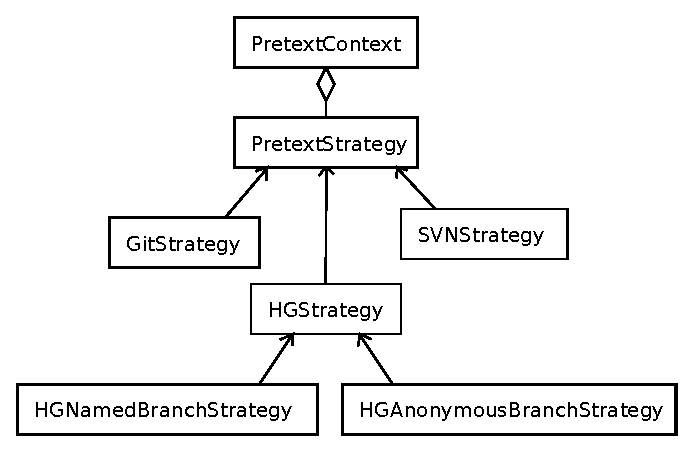
\includegraphics[width=\textwidth/2]{img/uml.eps}
	\caption{Diagram of our initial architecture.}
	\label{fig:architecture}
\end{figure}

One of the key decisions in the design of our product is how to accommodate the
support of additional SCMs.

Our goal is to make the implementation as general as possible, and thus to
minimize the work to be done by the SCM-specific parts of the code.
To do this we ned to make an abstraction of the actions that we need to perform
on the SCM workspace.
As the most important SCMs we have to support are distributed SCMs, we have
mostly considered these, and support for systems such as SVN will be considered
later in the process.
Luckily, the actions that we need to perform are all quite simple, so the
transition to other systems will most likely be painless.

The most challenging task is to accommodate the different ways people use their
SCMs.
For example, Mercurial users have drastically different ways of branching their
code; some use the actual branching command, some use anonymous branches, and
some use bookmarks to achieve the same result.
Because of this, we need to implement different schemes not only for different
SCMs but also for the different ways people use them.
At this early stage of development we will only implement support for one of the
branching methods in Mercurial, but the challenge is to make sure that the
design will accommodate the other later.

To be able to implement separate logic for each SCM and branching method we have
created a design using the strategy pattern, see figure \ref{fig:architecture}.
By specifying an interface for the strategy we have a single way of
communicating with the strategies, so the change of SCM will be completely
seamless for the rest of our program.

\end{document}
